\chapter{Colmenarejo and Nature}
\vspace{0.6cm}
\begin{center}
\nopagebreak
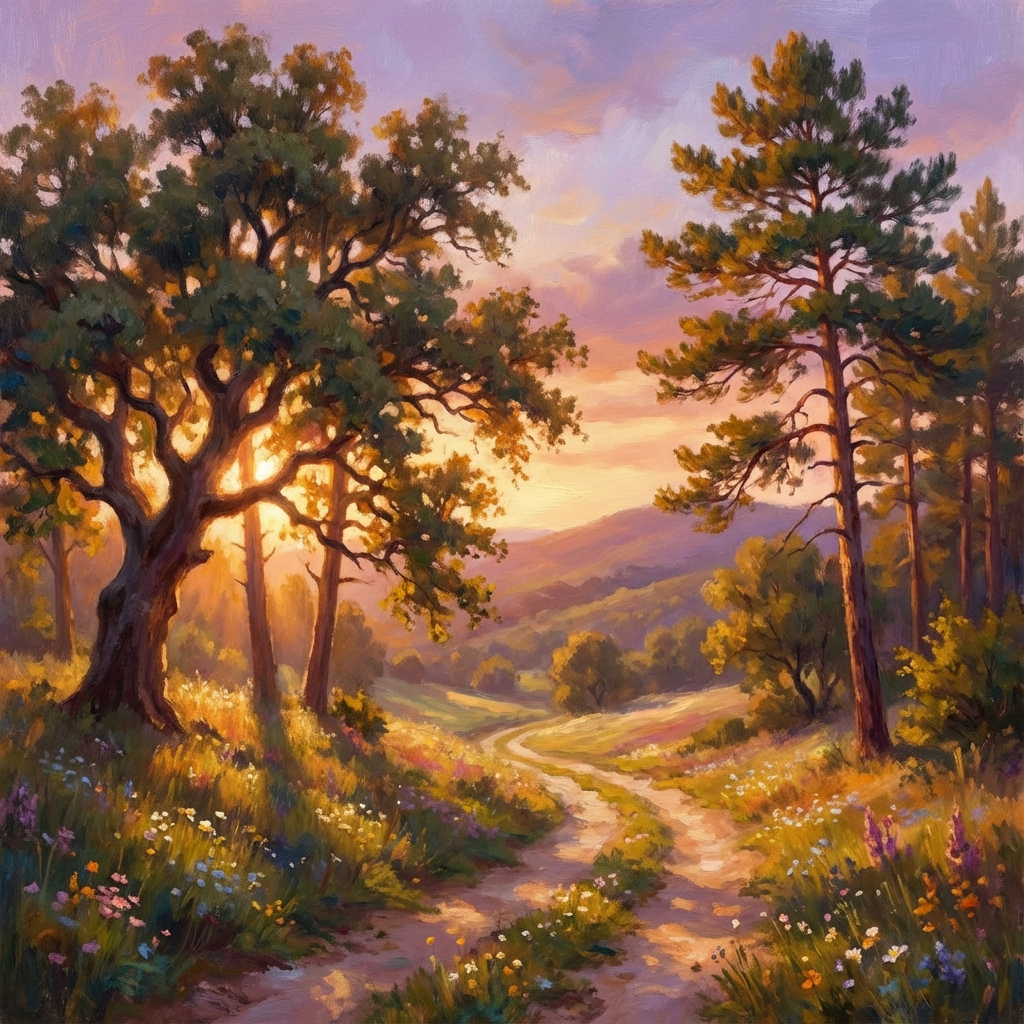
\includegraphics[width=0.75\textwidth,cfbox=gray!60 0.6pt 4pt]{nature.png}\\
\vspace{4pt}
{\small\itshape Surrender and peace: the natural flow of Being.}
\end{center}

\vspace{0.6cm}
We arrived in Colmenarejo at sunset. The town had that charm of what is halfway between the city and the countryside. We went towards the University area, where there are large open spaces and a different air is breathed.


—It feels better here —Jesus said, breathing deeply—. Nature is the great teacher of vibration. She is never wrong. A pine tree doesn't try to be a holm oak. A river doesn't try to flow upwards.


We sat near the hermitage. The sky was tinged with orange and violet.
—Our Father, who art in heaven... —he began to recite softly—. Do you know where heaven is, Francisco?


—Up there? —I pointed.


He shook his head, smiling.
—Heaven is a state of consciousness. It is that inner place where everything is fine, where there is absolute peace. ``Who art in heaven'' means that the Source of everything resides in that high vibration. And you have direct access there. You have direct wifi with the Creator, but sometimes you forget the password.


—What is the password?


—Surrender. Stop fighting against what is. Accept. Flow. When you surrender to life, you stop swimming against the current. And then, the current carries you. And the current of life always carries you towards the good, towards the sea.


In Colmenarejo, under the first stars, I understood that praying was not asking for things like someone making a shopping list. Praying was tuning in. It was putting the dial back on the correct frequency to listen to the music that is always playing, even though we are too busy making noise to hear it.